\documentclass[11pt,letterpaper]{article}
\usepackage[lmargin=1in,rmargin=1in,tmargin=1in,bmargin=1in]{geometry}
\usepackage{../style/homework}
\usepackage{../style/commands}
\setbool{quotetype}{false} % True: Side; False: Under
\setbool{hideans}{false} % Student: True; Instructor: False

% -------------------
% Content
% -------------------
\begin{document}

\homework{6: Due 02/24}{Honey, it's just the way your brain was hardwired. Plenty of great, intelligent, funny, interesting, and creative people have struggled with the same things you struggle with.}{Leslie Bennett, Euphoria}

% Problem 1
\problem{10} Determine if the relations $f(x)$ and $g(x)$ shown below are functions. Explain why or why not. If the relation is a function, determine its domain, codomain, and range. 
	\[
	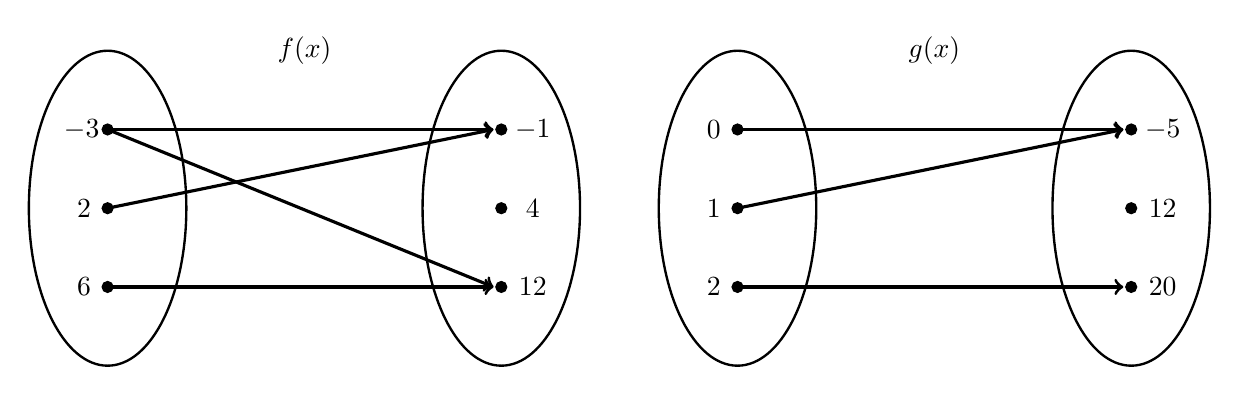
\begin{tikzpicture}
	\node at (2.5,2) {$f(x)$};
	% Ellipses
	\draw[line width=0.03cm] (0,0) circle (1 and 2);
	\draw[line width=0.03cm] (5,0) circle (1 and 2);
	
	% Nodes
	\draw[fill=black] (0,1) circle (0.07);
	\draw[fill=black] (0,0) circle (0.07);
	\draw[fill=black] (0,-1) circle (0.07);
	
	\draw[fill=black] (5,1) circle (0.07);
	\draw[fill=black] (5,0) circle (0.07);
	\draw[fill=black] (5,-1) circle (0.07);
	
	% Arrow
	\draw[line width=0.04cm,->] (0,1) -- (4.9,1);
	\draw[line width=0.04cm,->] (0,1) -- (4.9,-1);
	\draw[line width=0.04cm,->] (0,0) -- (4.9,1);
	\draw[line width=0.04cm,->] (0,-1) -- (4.9,-1);
	
	% Labels
	\node at (-0.3,1) {$\!-3$};
	\node at (-0.3,0) {$2$};
	\node at (-0.3,-1) {$6$};
	
	\node at (5.4,1) {$-1$};
	\node at (5.4,0) {$4$};
	\node at (5.4,-1) {$12$};
	
	\tikzset{shift={(8,0)}}
	%
	\node at (2.5,2) {$g(x)$};
	% Ellipses
	\draw[line width=0.03cm] (0,0) circle (1 and 2);
	\draw[line width=0.03cm] (5,0) circle (1 and 2);
	
	% Nodes
	\draw[fill=black] (0,1) circle (0.07);
	\draw[fill=black] (0,0) circle (0.07);
	\draw[fill=black] (0,-1) circle (0.07);
	
	\draw[fill=black] (5,1) circle (0.07);
	\draw[fill=black] (5,0) circle (0.07);
	\draw[fill=black] (5,-1) circle (0.07);
	
	% Arrow
	\draw[line width=0.04cm,->] (0,1) -- (4.9,1);
	\draw[line width=0.04cm,->] (0,0) -- (4.9,1);
	\draw[line width=0.04cm,->] (0,-1) -- (4.9,-1);
	
	% Labels
	\node at (-0.3,1) {$0$};
	\node at (-0.3,0) {$1$};
	\node at (-0.3,-1) {$2$};
	
	\node at (5.4,1) {$-5$};
	\node at (5.4,0) {$12$};
	\node at (5.4,-1) {$20$};
	\end{tikzpicture}
	\] \pspace

\sol The relation $f(x)$ is \textit{not} a function---$f(-3)$ is not well defined, i.e. the input $-3$ has two possible outputs. If it were a function, it would have domain $\{ -3, 2, 6 \}$, codomain $\{-1, 4, 12 \}$, and range $\{ -1, 12 \}$. \pspace

The relation $g(x)$ is a function---each possible input has only one possible output. The domain of $g(x)$ is $\{ 0, 1, 2 \}$, the codomain is $\{ -5, 12, 20 \}$, and the range is $\{ -5, 20 \}$. 



\newpage



% Problem 2
\problem{10} Determine if the relations $f(x)$ and $g(x)$ shown below are functions. Explain why or why not. If the relation is a function, compute the functions value at $x= 10$. 
	\[
	\begin{aligned}
	f(x)&= 47.3 - 17.9x \\[0.3cm]
	g(x)&= 2x^2 + 5x - 6
	\end{aligned}
	\] \pspace

\sol Both the relations $f(x)$ and $g(x)$ are functions---for each input, there is only one possible output. Namely, the output is obtained by evaluating at $x= x_0$ and following order of operations. Now we find $f(10)$ and $g(10)$: \pspace
	\[
	\begin{aligned}
	f(10)&= 47.3 - 17.9(10)= 47.3 - 1.79= -131.7 \\[0.3cm]
	g(10)&= 2(10^2) + 5(10) - 6= 2(100) + 5(10) - 6= 200 + 50 - 6= 244
	\end{aligned}
	\]



\newpage



% Problem 3
\problem{10} Suppose $f(x)$ and $g(x)$ are the functions given below. 
        \begin{table}[!ht]
        \centering
        \begin{tabular}{| c || c | c | c | c | c | c | c |} \hline
	$x$ & $-3$ & $-2$ & $-1$ & $\phantom{-}0$ & $\phantom{-}1$ & $\phantom{-}2$ & $\phantom{-}3$ \\ \hline
	$f(x)$ & $5$ & $2$ & $0$ & $-1$ & $-2$ & $-4$ & $-5$ \\ \hline
	$g(x)$ & $1$ & $1$ & $5$ & $2$ & $-3$ & $-3$ & $4$ \\ \hline
	$h(x)$ & $-6$ & $7$ & $1$ & $-2$ & $0$ & $1$ & $-1$ \\ \hline
        \end{tabular}
        \end{table}

Compute the following: \pspace
        \begin{enumerate}[(a)]
        \item $(f + g)(3)= f(3) + g(3)= -5 + 4= -1$ \vfill
        \item $(f - g)(-1)= f(-1) - g(-1)= 0 - 5= -5$ \vfill
        \item $(5h)(1)= 5h(1)= 5(0)= 0$ \vfill
        \item $\left(\dfrac{h}{g}\right)(-3)= \dfrac{h(-3)}{g(-3)}= \dfrac{-6}{1}= -6$ \vfill
        \item $f(2)\, h(-2)= -4 \cdot 7= -28$ \vfill
        \item $h(-1 - f(0))= h(-1 - (-1))= h(0)= -2$ \vfill
        \item $(g \circ f)(-2)= g(f(-2))= g(2)= -3$ \vfill
	\item $(h \circ g)(1)= h(g(1))= h(-3)= -6$ \vfill
        \item $(g \circ h)(1)= g(h(1))= g(0)= 2$ \vfill
	\item $(g \circ f \circ h)(-1)= g(f(h(-1)))= g(f(1))= g(-2)= 1$ \vfill
        \end{enumerate} \pspace



\newpage



% Problem 4
\problem{10} Suppose $f(x)$ and $g(x)$ are the functions given below. 
	\[
	\begin{aligned}
	f(x)&= 3x - 10 \\[0.3cm]
	g(x)&= 2x^2 - x + 5
	\end{aligned}
	\]

Compute the following: \pspace
\begin{enumerate}[(a)]
\item $f(3)= 3(3) - 10= 9 - 10= -1$ \vfill
\item $g(-2)= 2(-2)^2 - (-2) + 5= 2(4) + 2 + 5= 8 + 2 + 5= 15$ \vfill
\item $5f(6) - g(1)= 5 (3 \cdot 6 - 10) - (2 \cdot 1^2 - 1 + 5)= 40 - 6= 34$ \vfill
\item $f(x) - g(x)= (3x - 10) - (2x^2 - x + 5)= 3x - 10 - 2x^2 + x - 5= -2x^2 +4x -15 $ \vfill
\item $f(x) \, g(x)= (3x - 10)(2x^2 - x + 5)= 6x^3 - 3x^2 + 15x - 20x^2 + 10x - 50= 6x^3 - 23x^2 + 25x - 50$ \vfill
\item $\left( \dfrac{f}{g} \right)(x)=\dfrac{3x - 10}{2x^2 - x + 5}$ \vfill
\item $(f \circ g)(0)= f(g(0))= f(2 \cdot 0^2 - 0 + 5)= f(5)= 3(5) - 10= 5$ \vfill
\item $(g \circ f)(3)= g(f(3))= g(3 \cdot 3 - 10)= g(-1)= 2(-1)^2 - (-1) + 5= 2 + 1 + 5= 8$ \vfill
\item $(f \circ g)(x)= f(g(x))= f(2x^2 - x + 5)= 3(2x^2 - x + 5) - 10= 6x^2 - 3x + 15 - 10= 6x^2 - 3x + 5$ \vfill
\item $(g \circ f)(x)= g(f(x))= g(3x - 10)= 2(3x - 10)^2 - (3x - 10) + 5= 18x^2 - 123x + 215$ \vfill
\end{enumerate} \pspace



\newpage



% Problem 5
\problem{10} Determine if the relation below is a function or not. If it is a function, explain why. If it is not a function, explain why. Determine also whether the relation has an inverse function. If it has an inverse function, explain why. If it does not have an inverse function, explain why not. 
	\[
	\fbox{
	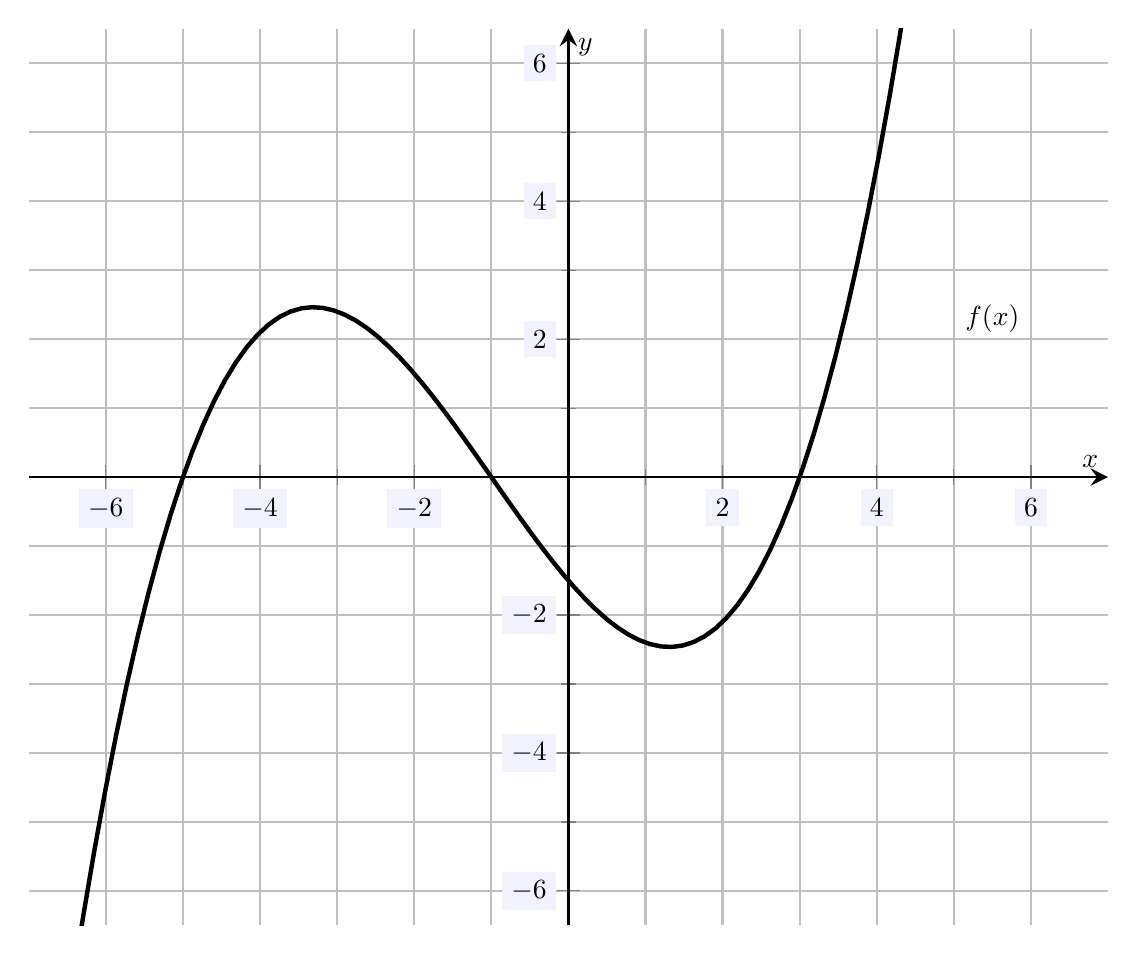
\begin{tikzpicture}[scale=2,every node/.style={scale=0.5}]
	\begin{axis}[
	grid=both,
	axis lines=middle,
	ticklabel style={fill=blue!5!white},
	xmin= -7, xmax=7,
	ymin= -6.5, ymax=6.5,
	xtick={-6,-4,-2,0,2,4,6},
	ytick={-6,-4,-2,0,2,4,6},
	minor tick = {-5,-3,...,5},
	xlabel=\(x\),ylabel=\(y\),
	]
	\node at (5.5,2.3) {$f(x)$};
	\addplot[thick, domain= -7:7, samples=100] ({x},{1/10*(x + 5)*(x + 1)*(x - 3)});
	\end{axis}
	\end{tikzpicture}
	}
	\] \pspace

\sol The relation \textit{is} a function because it passes the vertical line test, i.e. every vertical line intersects the curve in at most one point. However, the relation \textit{does not} have an inverse because it fails the horizontal line test, i.e. not every horizontal line intersects the curve in at most one point. For instance, the horizontal line $y= 0$ intersects the curve at the point $(-5, 0)$, $(-1, 0)$, $(3, 0)$. This implies that $f^{-1}(0)$ is not well defined so that $f^{-1}(x)$ cannot be a function. 



\newpage



% Problem 6
\problem{10} Determine whether the point $(2, -1)$ is on the graph of $f(x)= 2x^2 - 5x + 3$. Determine also whether the point $(1, 0)$ is on the graph of $f(x)$. For each, explain why or why not. \pspace

\sol If $(x, y)= (2, -1)$ is on the curve $f(x)= 2x^2 - 5x + 3$, then when $x= 2$, $y= -1$, i.e. $f(2)= -1$, which we check:
	\[
	f(2)= 2(2^2) - 5(2) + 3= 2 \cdot 4 - 5(2) + 3= 8 - 10 + 3= 1 
	\]
Because $f(2)= 1 \neq -1$, the point $(2, -1)$ is \textit{not} on the graph of $f(x)$. We repeat the same process for $(x, y)= (1, 0)$:
	\[
	f(1)= 2(1^2) - 5(1) + 3= 2 \cdot 1 - 5(1) + 3= 2 - 5 + 3= 0 
	\]
Therefore, $(1, 0)$ \textit{is} on the graph of $f(x)$. 


\end{document}